\documentclass{article}
\usepackage[ a4 paper, margin=1in,bottom=2in  ]{ geometry }
\usepackage{ amsmath , amssymb , mathtools } % math
\usepackage{ booktabs , multirow , array } % pro tables
\usepackage[ table ]{ xcolor } % colors + colored table rows
\usepackage{ listings } % code listings
\usepackage{ wrapfig , rotating , graphicx } % figures
\usepackage[ shortlabels ]{ enumitem } % custom lists
\usepackage[ colorlinks = false ]{ hyperref } % links + \ url + \ href
\usepackage{float}
\graphicspath{ {.} } 

\hypersetup{
    colorlinks=true,
    urlcolor=blue,
    linkcolor=black,
    citecolor=black
}


\title{\textbf{Laplace Analysis and Applications}}
\author{
  Pierre-Simon Laplace\textsuperscript{1},Oliver Heaviside\textsuperscript{2}, 
  and Gustav Robert Kirchhoff\textsuperscript{3}
}
\date{}
\begin{document}
\maketitle

\begin{center}
\textsuperscript{1}Acad\'emie des Sciences, Paris, France\\
\textsuperscript{2}Royal Society, London, United Kingdom\\
\textsuperscript{3}University of Heidelberg, Heidelberg, Germany
\end{center}

\section{From Functions to Transforms}
\subsection{The Laplace Transform}

Let $f(t)$ be a function defined for $ t \geq 0$. Its Laplace transform is defined by
\begin{equation}
    \mathcal{L}\{f(t)\}= F(s) = \int_{0}^{\infty} e^{st}f(t) \,dt|,
     \qquad s>0. 
\end{equation}
The transform changes a function of time into a function of the new variable 
$s$.\footnote[1]{The variable $s$ is commonly interpreted as a complex-frequency variable.} Symbolically,
\begin{displaymath}
    f(t) \quad \xrightarrow{\mathcal{L}} \quad F(s).
\end{displaymath}

The inverse Laplace transform reverses this process:
\begin{equation}
    f(t)= \mathcal{L}^{-1}\{F(s)\}.
\end{equation}
The main purpose of the method is to replace differentiation and integration in the time domain
by simpler algebraic operations in the transform domain [1]. A concise overview is available from the \href{https://mathworld.wolfram.com/LaplaceTransform.html}{Laplace Transform on Mathworld} 
entry on MathWorld.
\subsection{A simple Example}

For the constant function $f(t)= 1$,

\begin{align}
    \mathcal{L} &=\int_{0}^{\infty} e^{-st}dt \nonumber \\
    &=\left[- \frac{1}{s}e^{-st}\right]_{0}^{\infty} \nonumber \\
    &= \frac{1}{s}
\end{align}
Similarly,
\begin{equation}
    \mathcal{L}= \frac{1}{s^2}, \qquad \mathcal{L}=\frac{2}{s^3}.
\end{equation}
\newpage
\section{Common Transform Equations}
Table 1 lists several frequently used Laplace-transform equations.
\begin{table}[H]
    \centering
    \renewcommand{\arraystretch}{1.5}
    \caption{Selected Laplace-transform equations.}\label{tab:laplace}
    \begin{tabular}{|c|c|c|c|}
        \hline
        \multirow{2}{*}{\textbf{Family}} 
        & \multicolumn{2}{c|}{\textbf{Transform Equation}} 
        & \multirow{2}{*}{\textbf{Condition}} \\
        \cline{2-3}
        &  \textbf{Time Funtion} & \textbf{Laplace transform} & \\
        \hline
        \multirow{3}{*}{Algebraic} 
        & $1$ & $\frac{1}{s}$ & $ s>0$ \\
        \cline{2-4}
        &$t$ & $\frac{1}{s^2}$ & $s>0$ \\
        \cline{2-4}
        & $t^n$ & $\frac{n!}{s^{n+1}}$ & $ n=0,1,2,\dots$ \\
        \hline
        \multirow{2}{*}{Exponential} & $e^{at}$ & $\frac{1}{x-a}$ & $s>a$ \\
        \cline{2-4}
        & $e^{-at}$ & $\frac{1}{s+a}$ & $s>-a$ \\
        \hline
        \multirow{2}{*}{Oscillatory} & $\sin(\omega t)$
        & $\frac{\omega}{s^2 + \omega^2}$ & $\omega > 0 $ \\
        \cline{2-4}
        & $\cos(\omega t)$
        & $\frac{s}{s^2 + \omega^2}$ & $\omega > 0 $ \\
        \hline
        \multicolumn{2}{|c|}{\textbf{Unit-step function} $u(t-a)$} &
        $\frac{e^{-as}}{s}$ & $a>0$ \\
        \hline

    \end{tabular}
    
\end{table}

    The formulas in Table \ref{tab:laplace} allow many functions to be transformed without repeatedly evaluating
improper integrals.

\section{Application to an RC Circuit}
\subsection*{Circuit Model}
\begin{wrapfigure}{r}{0.5\textwidth}
    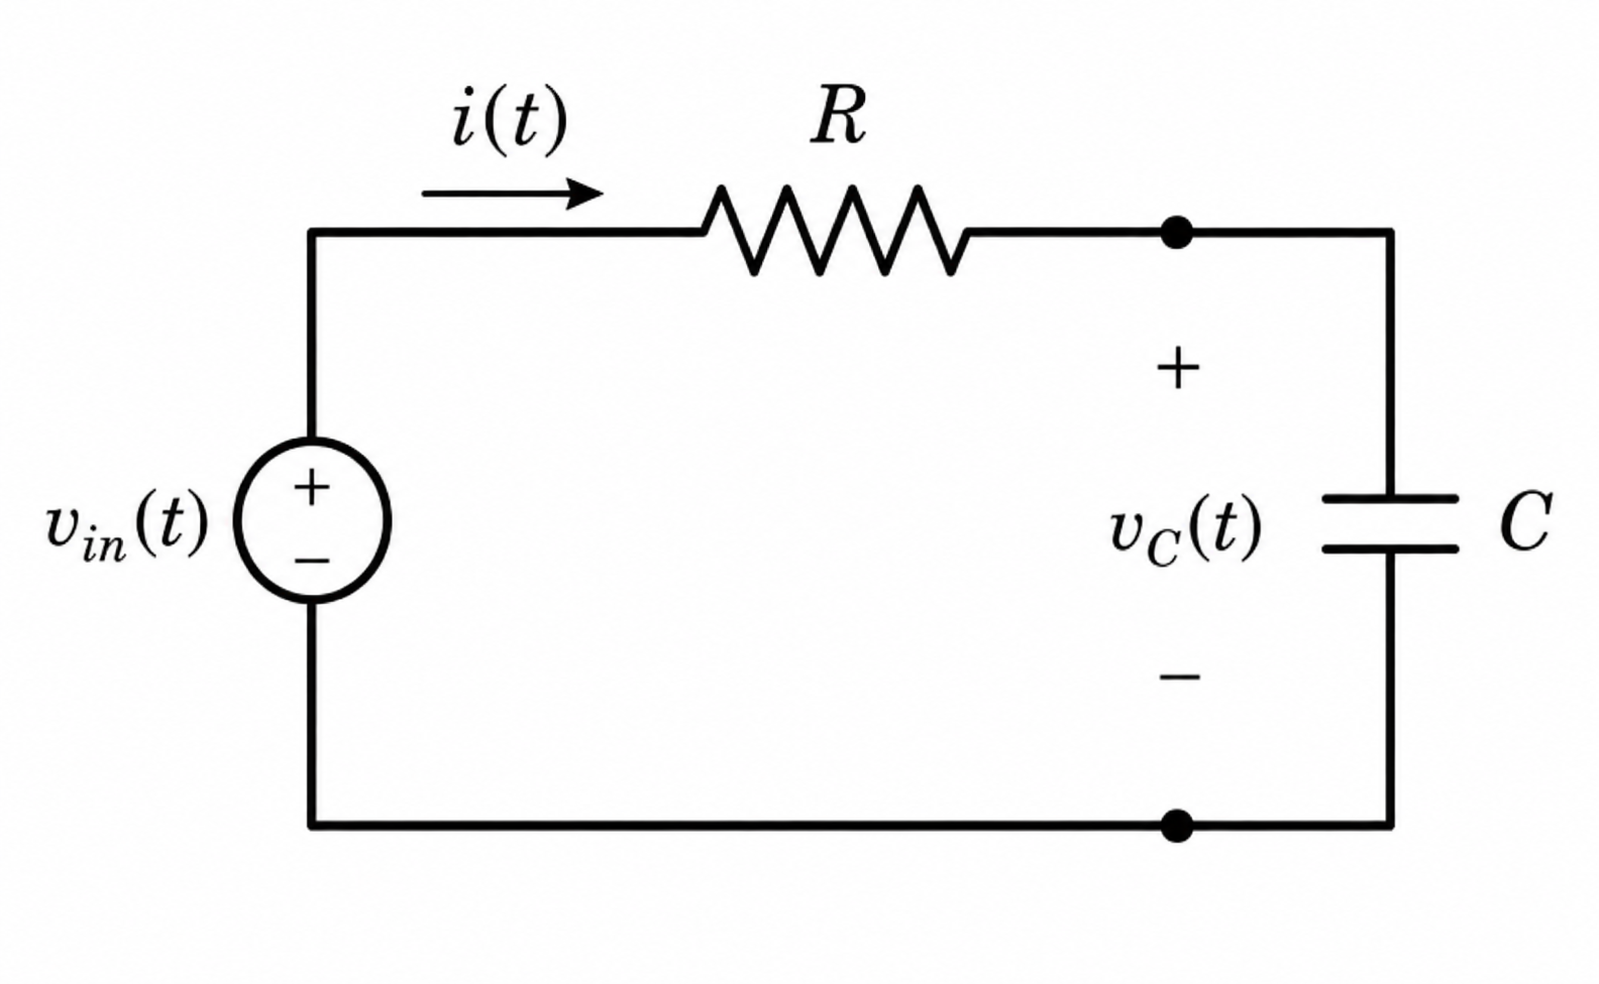
\includegraphics[width=\linewidth]{rc_circuit.png}
    \caption{A simple series RC circuit.}
    \label{fig:rc_circuit}
\end{wrapfigure}
Figure 1 shows a simple \texttt{resistor--capacitor
circuit} connected to an input voltage source.
The resistor limits the current, while the capacitor
stores electrical energy.

For a resistor $R$ and capacitor $C$, Kirchhoff’s
voltage law gives
\begin{equation}
    RC \frac{dv_c(t)}{dt} + v_c(t) = v_{in}t,
\end{equation}
where $v_c(t) $ is the voltage across the capacitor.

Assuming $v_c(0)=0$ taking the Laplace transform of Equation (5) gives
\end{document}